\documentclass[conference]{IEEEtran}
\IEEEoverridecommandlockouts

% Configuración para español
\usepackage[spanish,es-nodecimaldot,es-noshorthands]{babel}
\usepackage[utf8]{inputenc}
\usepackage[T1]{fontenc}

% Paquetes estándar IEEE
\usepackage{cite}
\usepackage{amsmath,amssymb,amsfonts}
\usepackage{algorithmic}
\usepackage{graphicx}
\usepackage{textcomp}
\usepackage{xcolor}
\usepackage{float}
\usepackage{listings} % Para código
\usepackage{url}

% ---------- Configuración de listados de código ----------
\definecolor{codegray}{rgb}{0.45,0.45,0.45}
\definecolor{codeblue}{rgb}{0.10,0.10,0.60}
\definecolor{codegreen}{rgb}{0.1,0.5,0.1}
\lstset{
	basicstyle=\ttfamily\scriptsize,
	keywordstyle=\color{codeblue}\bfseries,
	commentstyle=\color{codegreen}\itshape,
	stringstyle=\color{codegray},
	numbers=left,
	numberstyle=\tiny\color{codegray},
	numbersep=5pt,
	frame=single,
	breaklines=true,
	breakatwhitespace=true,
	showstringspaces=false,
	tabsize=2,
	captionpos=b,
	literate=%
	{á}{{\'a}}1 {é}{{\'e}}1 {í}{{\'i}}1 {ó}{{\'o}}1 {ú}{{\'u}}1
	{Á}{{\'A}}1 {É}{{\'E}}1 {Í}{{\'I}}1 {Ó}{{\'O}}1 {Ú}{{\'U}}1
	{ñ}{{\~n}}1 {Ñ}{{\~N}}1 {¿}{{?`}}1 {¡}{{!`}}1
}

\def\BibTeX{{\rm B\kern-.05em{\sc i\kern-.025em b}\kern-.08em
	T\kern-.1667em\lower.7ex\hbox{E}\kern-.125emX}}

\begin{document}

\title{Práctica 9: IDE y Depuración en Sistemas Embebidos}

\author{
	\IEEEauthorblockN{Belmont Muñoz Samuel}
	\IEEEauthorblockA{\textit{Ingeniería en Computación} \\
		\textit{Facultad de Ingeniería}\\
		No. Cuenta: 317318289}
	\and
	\IEEEauthorblockN{Domínguez Palacios Jesús Alejandro}
	\IEEEauthorblockA{\textit{Ingeniería en Computación} \\
		\textit{Facultad de Ingeniería}\\
		No. Cuenta: 421066205}
	\and
	\IEEEauthorblockN{Dorantes Mejía Emmanuel}
	\IEEEauthorblockA{\textit{Ingeniería en Computación} \\
		\textit{Facultad de Ingeniería}\\
		No. Cuenta: 313004766}
	\and
	\IEEEauthorblockN{García Olvera Emiliano}
	\IEEEauthorblockA{\textit{Ingeniería en Computación} \\
		\textit{Facultad de Ingeniería}\\
		No. Cuenta: 314256009}
	\and
	\IEEEauthorblockN{Hernández Alonso Antonio Adonahí}
	\IEEEauthorblockA{\textit{Ingeniería en Computación} \\
		\textit{Facultad de Ingeniería}\\
		No. Cuenta: 320257780}
	\and
	\IEEEauthorblockN{Jiménez Reyes Alan Yael}
	\IEEEauthorblockA{\textit{Ingeniería en Computación} \\
		\textit{Facultad de Ingeniería}\\
		No. Cuenta: 320026726}
}

\maketitle

\begin{center}
	\vspace{-0.3cm}
	{\small
		\textbf{Práctica No.:} 9 \quad | \quad
		\textbf{Grupo:} 6 \quad | \quad
		\textbf{Fecha:} 26/10/2026
	}
	\vspace{0.2cm}
\end{center}

\begin{abstract}
	Este reporte documenta el uso de herramientas de depuración (\textit{debugging}) para programas en C ejecutados sobre una Raspberry Pi 4. Se utilizó \texttt{gdb} en terminal para controlar la ejecución, inspeccionar variables y analizar la pila de llamadas mediante \textit{breakpoints} y \textit{watchpoints}, incluyendo el modo TUI. Posteriormente, se integró el entorno de Visual Studio Code mediante Remote-SSH para depurar gráficamente. Se utilizó \texttt{gdbserver} para separar el depurador del proceso en ejecución. El trabajo permitió diagnosticar tres fallas típicas (desreferenciación nula, bucle infinito y corrupción de memoria) y culminó con la corrección de tres defectos lógicos y estructurales en un programa simulado (\texttt{averiado.c}), demostrando la importancia del análisis paso a paso en sistemas embebidos.
\end{abstract}

\begin{IEEEkeywords}
	Depuración, gdb, gdbserver, VS Code, breakpoints, watchpoints, Raspberry Pi, sistemas embebidos
\end{IEEEkeywords}

% ---------------------------------------------------------
% SECCIÓN I: OBJETIVO (Debe ir antes de la Introducción)
% ---------------------------------------------------------
\section{Objetivo}

\subsection{Objetivo General}
Depurar con \texttt{gdb}, VS Code y \texttt{gdbserver} programas en C que corren en la Raspberry Pi, y aplicar esas herramientas para localizar y corregir defectos en un programa que no se conocía.

\subsection{Objetivos Específicos}
\begin{itemize}
	\item Compilar con información de depuración y sin optimización, y explicar qué cambia en el ejecutable.
	\item Controlar la ejecución con \textit{breakpoints}, condiciones, avance paso a paso y \textit{watchpoints}.
	\item Inspeccionar y modificar variables del Centinela mientras maneja el circuito.
	\item Diagnosticar una caída del programa, un ciclo que no termina y una corrupción de memoria.
	\item Configurar la depuración en VS Code sobre la Pi con \texttt{launch.json} y \texttt{tasks.json}.
	\item Conectar \texttt{gdb} a un programa a través de \texttt{gdbserver}.
\end{itemize}

% ---------------------------------------------------------
% SECCIÓN II: INTRODUCCIÓN
% ---------------------------------------------------------
\section{Introducción}

En el desarrollo de software para sistemas embebidos, el código interactúa directamente con el hardware, por lo que los errores pueden tener consecuencias físicas o dejar el sistema en un estado inoperable. La depuración (\textit{debugging}) es el proceso de identificar, aislar y corregir defectos en el software.

\subsection{Herramientas de Depuración}
\begin{itemize}
	\item \textbf{gdb (GNU Debugger)}: Permite ejecutar un programa paso a paso, inspeccionar el valor de las variables en memoria, ver la pila de llamadas (\textit{call stack}) y modificar el flujo de ejecución en tiempo real. Para que funcione, el binario debe compilarse con la bandera \texttt{-g} y preferiblemente sin optimizaciones (\texttt{-O0}). Cuenta además con el modo TUI (\textit{Text User Interface}) que permite ver el código fuente en pantalla dividida.
	\item \textbf{VS Code (Visual Studio Code)}: A través de la extensión \textit{Remote - SSH} y el depurador de C/C++, permite utilizar \texttt{gdb} de forma gráfica. Esto agiliza la inspección visual de variables (\textit{Watch}), la pila de llamadas y la configuración de puntos de interrupción directamente sobre el código fuente.
	\item \textbf{gdbserver}: Es un programa que corre en el sistema objetivo (la Raspberry Pi) y permite que un \texttt{gdb} remoto (en una laptop) se conecte a él mediante una red TCP. Es ideal cuando el sistema objetivo tiene recursos limitados o se encuentra en un entorno remoto.
\end{itemize}

\subsection{Conceptos Clave: Breakpoints y Watchpoints}
Un \textit{breakpoint} (punto de interrupción) detiene la ejecución del programa en una línea específica o al entrar a una función. Los \textit{breakpoints} condicionales solo detienen el programa si se cumple una expresión lógica. Por otro lado, un \textit{watchpoint} (punto de vigilancia) no se coloca en una línea de código, sino sobre una variable; el programa se detendrá automáticamente en el instante exacto en que el valor de esa variable cambie en memoria, lo cual es invaluable para detectar corrupciones silenciosas.

% ---------------------------------------------------------
% SECCIÓN III: DESARROLLO
% ---------------------------------------------------------
\section{Desarrollo}

\subsection{Parte A. Entorno y conexión}
Se verificó la arquitectura del sistema operativo (aarch64), así como las versiones de \texttt{gdb} (16.3) y \texttt{gdbserver} (16.3) instaladas en la Raspberry Pi. Se configuró el archivo \texttt{\textasciitilde/.gdbinit} para evitar la pregunta sobre \texttt{debuginfod} (Figura~\ref{fig:a1}). Posteriormente, se descomprimió el kit de trabajo (\texttt{FSE\_P09\_kit.zip}), se compiló con \texttt{make} y se abrió la carpeta remota \texttt{p09} desde una laptop mediante la extensión Remote-SSH de VS Code (Figuras~\ref{fig:a2} y \ref{fig:a3}).

\begin{figure}[!ht]
	\centering
	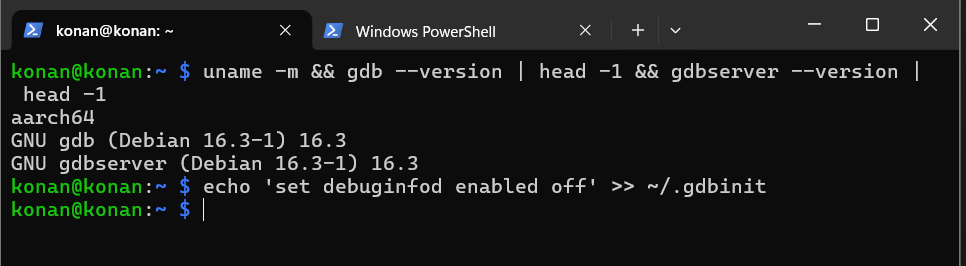
\includegraphics[width=0.9\columnwidth]{A_01_herramientas_versiones.png}
	\caption{Verificación de arquitectura, versiones de gdb/gdbserver y configuración de \texttt{.gdbinit}.}
	\label{fig:a1}
\end{figure}

\begin{figure}[!ht]
	\centering
	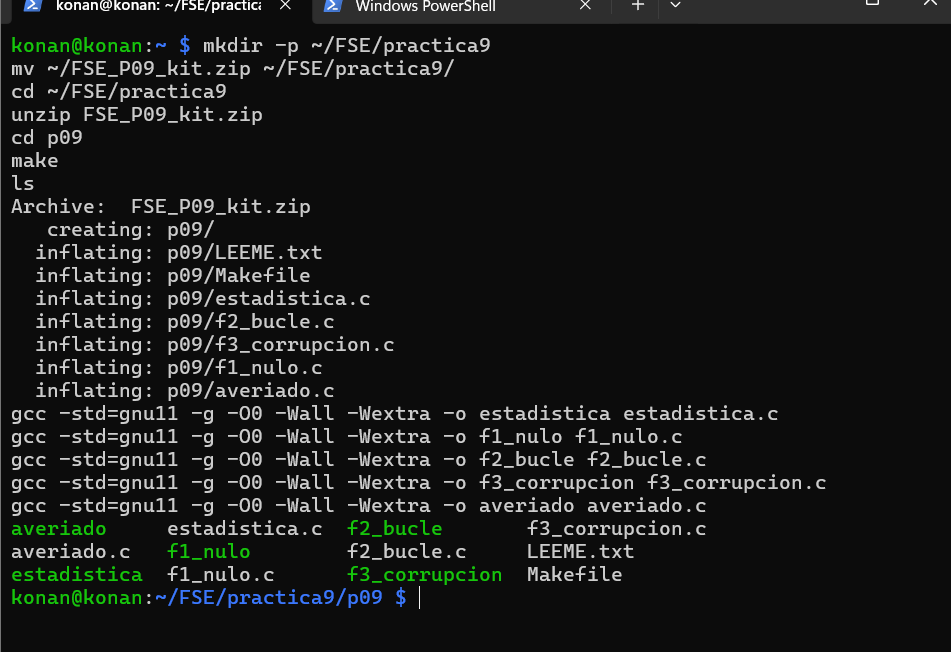
\includegraphics[width=0.9\columnwidth]{A_02_unzip_make_ls.png}
	\caption{Descompresión del kit, compilación con \texttt{make} y visualización de archivos generados.}
	\label{fig:a2}
\end{figure}

\begin{figure}[!ht]
	\centering
	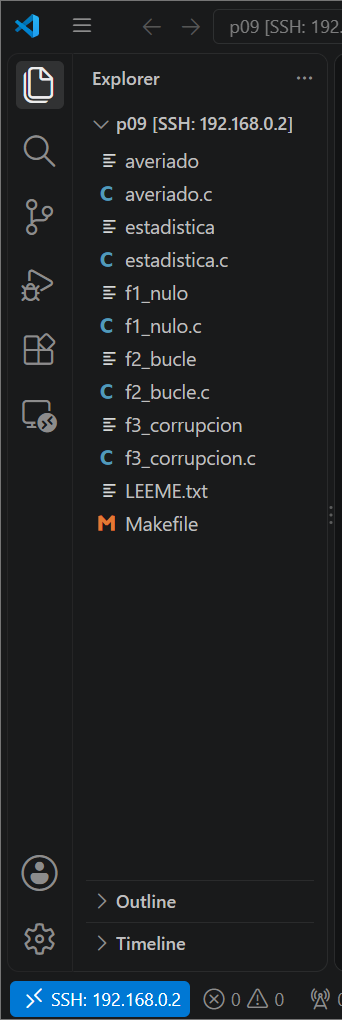
\includegraphics[height=7cm, keepaspectratio]{A_03_vscode_remote_ssh_p09.png}
	\caption{Conexión remota a la Raspberry Pi mediante VS Code y Remote-SSH.}
	\label{fig:a3}
\end{figure}

\subsection{Parte B. gdb en terminal}
Se depuró el programa \texttt{estadistica} para comprender el control de flujo. Se colocaron \textit{breakpoints} en la función \texttt{promedio}, se inspeccionó la pila con \texttt{bt} y los argumentos con \texttt{info args} (Figura~\ref{fig:b1}). Se probó la diferencia entre \texttt{next} y \texttt{step}. Al usar \texttt{finish}, el depurador terminó la ejecución de la función y devolvió el valor calculado (Figura~\ref{fig:b2}). Finalmente, se examinó el arreglo en memoria (Figura~\ref{fig:b3}), se usó \texttt{display total} (Figura~\ref{fig:b4}) y se colocó un \textit{watchpoint} en la variable \texttt{total} para detenerse cada vez que su valor cambiara (Figura~\ref{fig:b5}). También se utilizó la interfaz TUI de gdb para visualizar el código fuente (Figuras~\ref{fig:b6} y \ref{fig:b7}).

\begin{figure}[!ht]
	\centering
	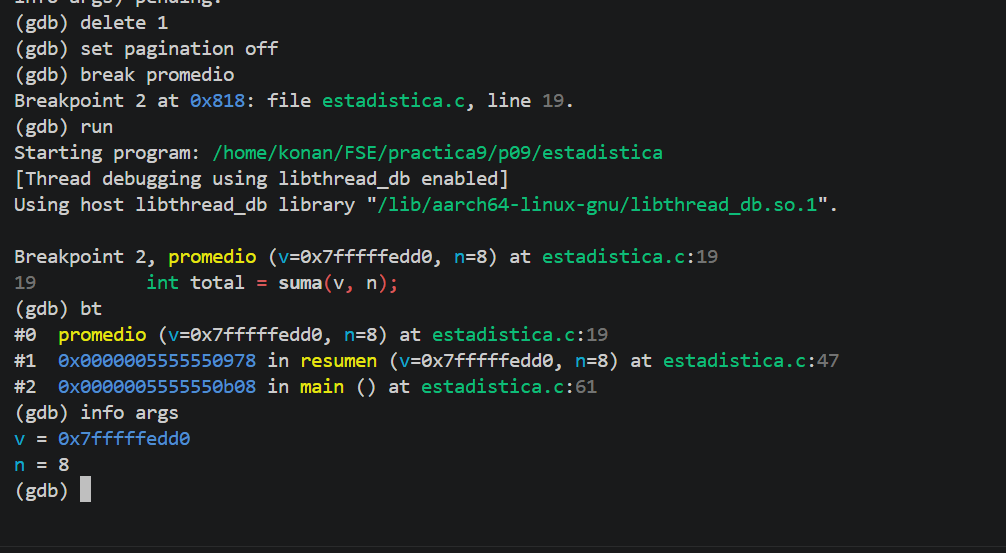
\includegraphics[width=0.9\columnwidth]{B_01_break_promedio_bt_info_args.png}
	\caption{Breakpoint en promedio, pila de llamadas (\texttt{bt}) y argumentos (\texttt{info args}).}
	\label{fig:b1}
\end{figure}

\begin{figure}[!ht]
	\centering
	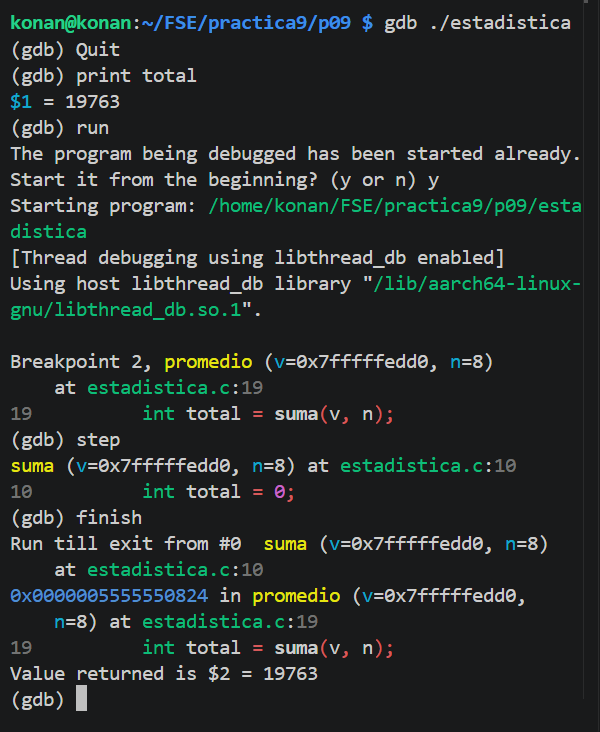
\includegraphics[width=0.9\columnwidth]{B_02_next_step_finish.png}
	\caption{Uso de \texttt{step} y \texttt{finish} para entrar y salir de la función \texttt{suma}.}
	\label{fig:b2}
\end{figure}

\begin{figure}[!ht]
	\centering
	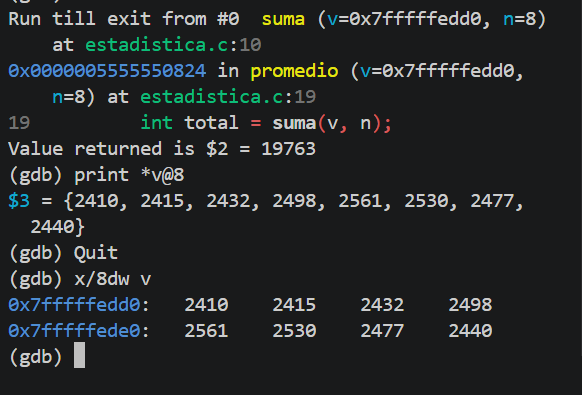
\includegraphics[width=0.9\columnwidth]{B_03_print_x_arreglo.png}
	\caption{Inspección del arreglo en memoria con \texttt{print *v@8} y \texttt{x/8dw v}.}
	\label{fig:b3}
\end{figure}

\begin{figure}[!ht]
	\centering
	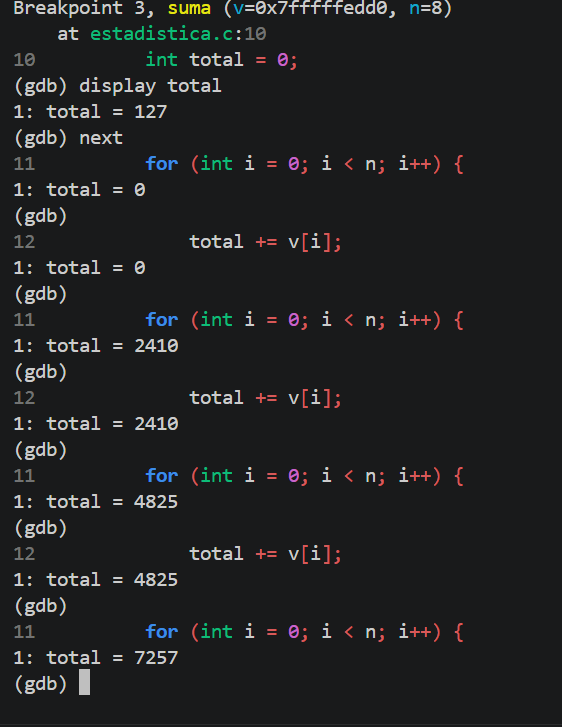
\includegraphics[width=0.9\columnwidth]{B_04_display_total.png}
	\caption{Comando \texttt{display total} y avance paso a paso observando los cambios de la variable.}
	\label{fig:b4}
\end{figure}

\begin{figure}[!ht]
	\centering
	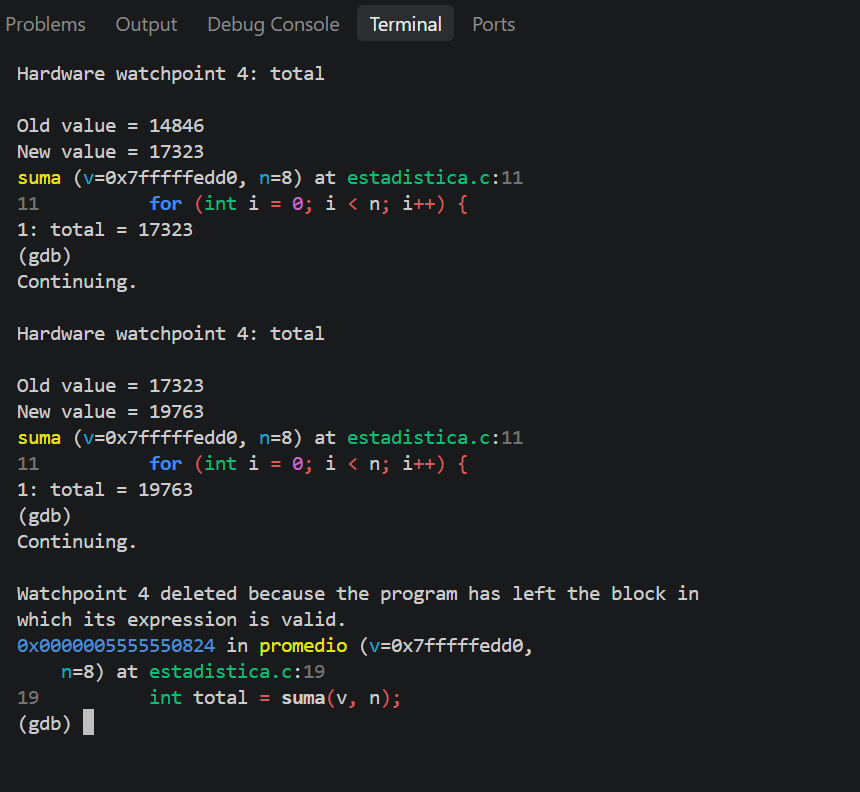
\includegraphics[width=0.9\columnwidth]{B_05_watch_total.png}
	\caption{Detenciones del watchpoint sobre la variable \texttt{total}.}
	\label{fig:b5}
\end{figure}

\begin{figure}[!ht]
	\centering
	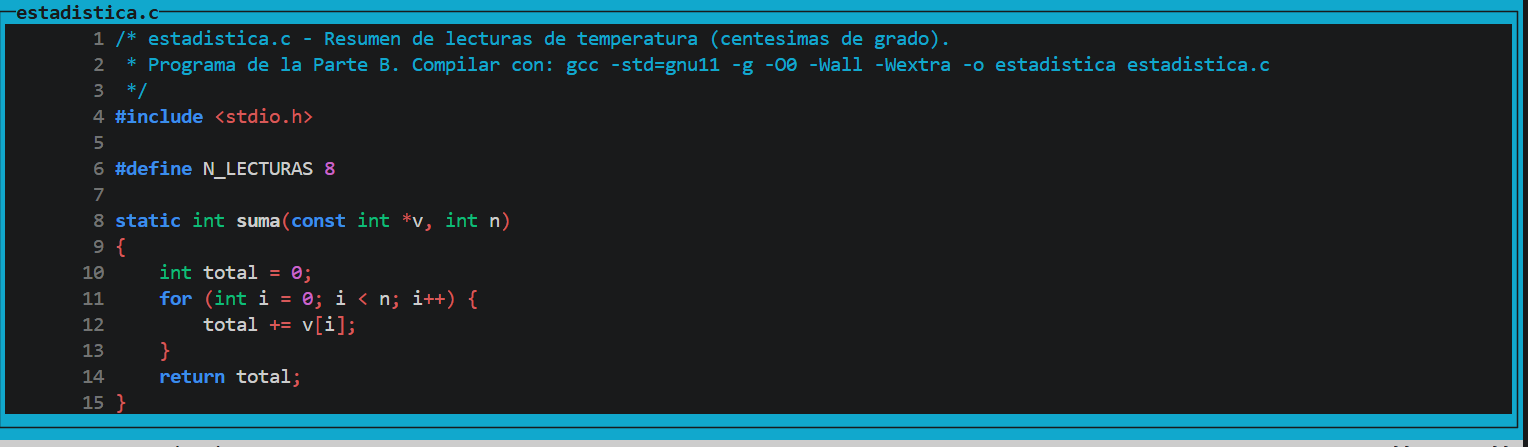
\includegraphics[width=0.9\columnwidth]{B_06_tui_suma.png}
	\caption{Interfaz TUI de gdb mostrando la función \texttt{suma}.}
	\label{fig:b6}
\end{figure}

\begin{figure}[!ht]
	\centering
	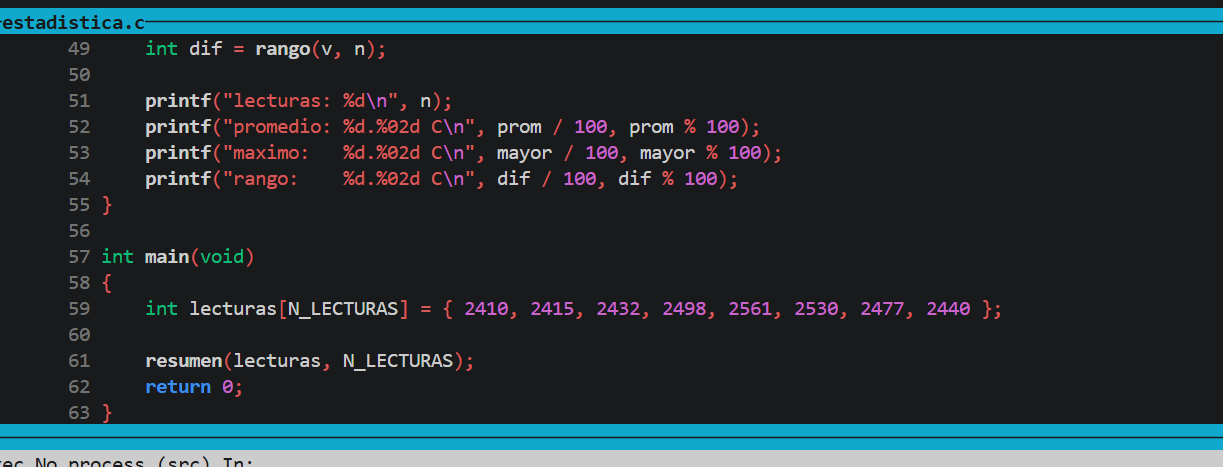
\includegraphics[width=0.9\columnwidth]{B_07_tui_main.png}
	\caption{Interfaz TUI de gdb mostrando la función \texttt{main}.}
	\label{fig:b7}
\end{figure}

\subsection{Parte C. Depurar el Centinela con el circuito}
Se compiló una copia para depurar (\texttt{centinela\_dbg}) y se utilizó \texttt{gdb} para forzar estados sin tocar el hardware. Se inspeccionaron los argumentos y la pila (Figura~\ref{fig:c1}). Utilizando \texttt{set var temp\_c100 = 3500}, se forzó la condición de alarma (Figura~\ref{fig:c2}) y se observó el comportamiento de los LEDs en la placa (Figura~\ref{fig:c3}). Se colocó un \textit{breakpoint} condicional para detenerse solo cuando el estado fuera \texttt{ALARMA} (Figura~\ref{fig:c4}). Se monitoreó el potenciómetro en sus límites (Figura~\ref{fig:c5}) y, mediante \texttt{watch estado}, se rastreó el cambio de estado global del Centinela a lo largo de la ejecución (Figuras~\ref{fig:c6} a \ref{fig:c8}).

\begin{figure}[!ht]
	\centering
	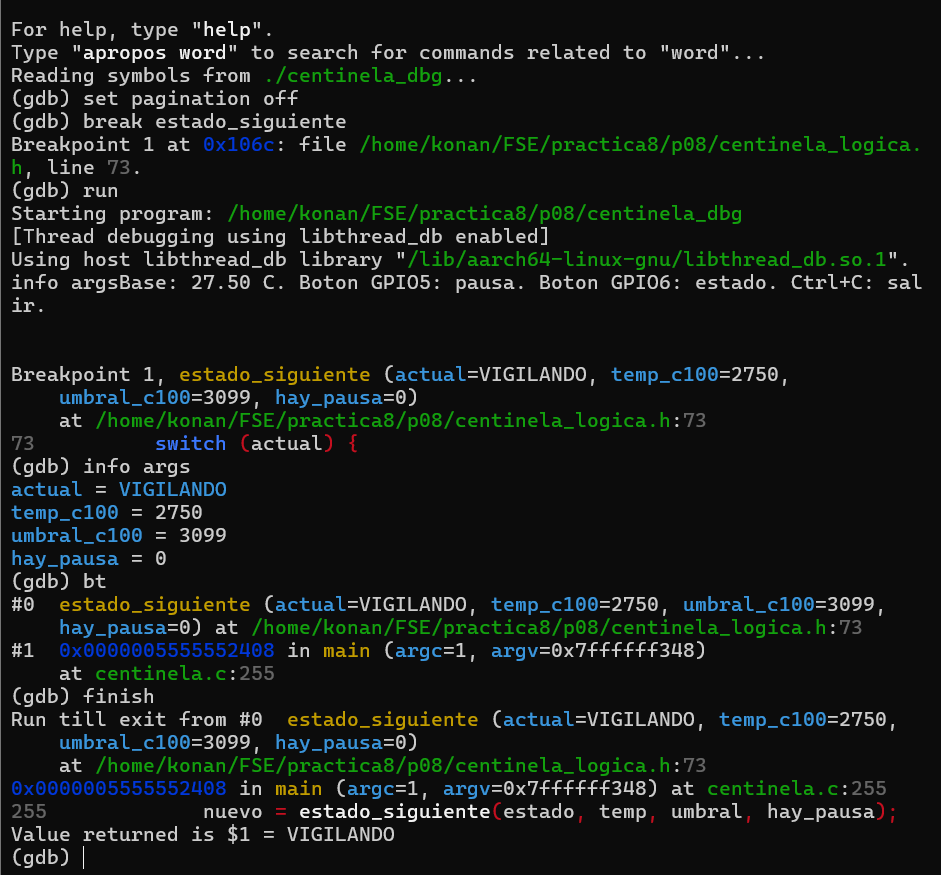
\includegraphics[width=0.9\columnwidth]{C_01_info_args_bt_finish.png}
	\caption{Inspección de argumentos y pila en el Centinela.}
	\label{fig:c1}
\end{figure}

\begin{figure}[!ht]
	\centering
	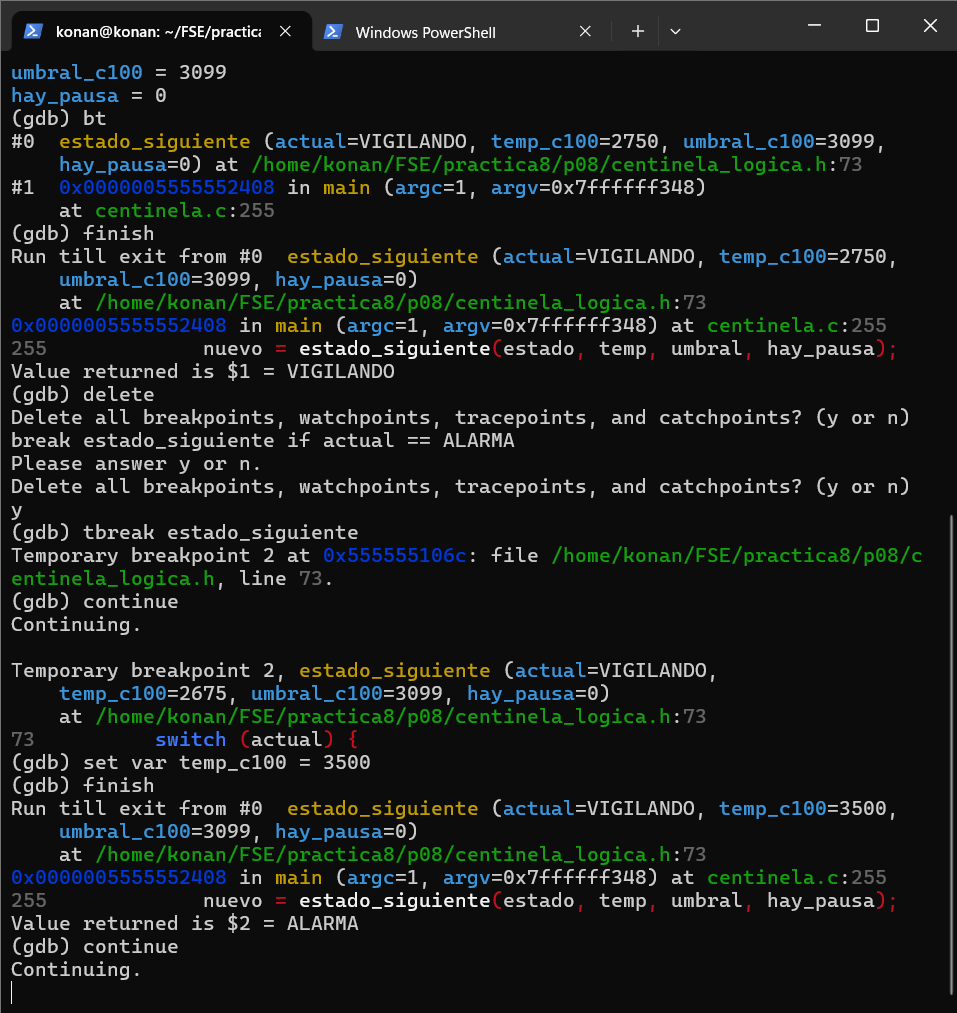
\includegraphics[width=0.9\columnwidth]{C_02_set_var_alarma.png}
	\caption{Modificación de la temperatura con \texttt{set var} para forzar el estado ALARMA.}
	\label{fig:c2}
\end{figure}

\begin{figure}[!ht]
	\centering
	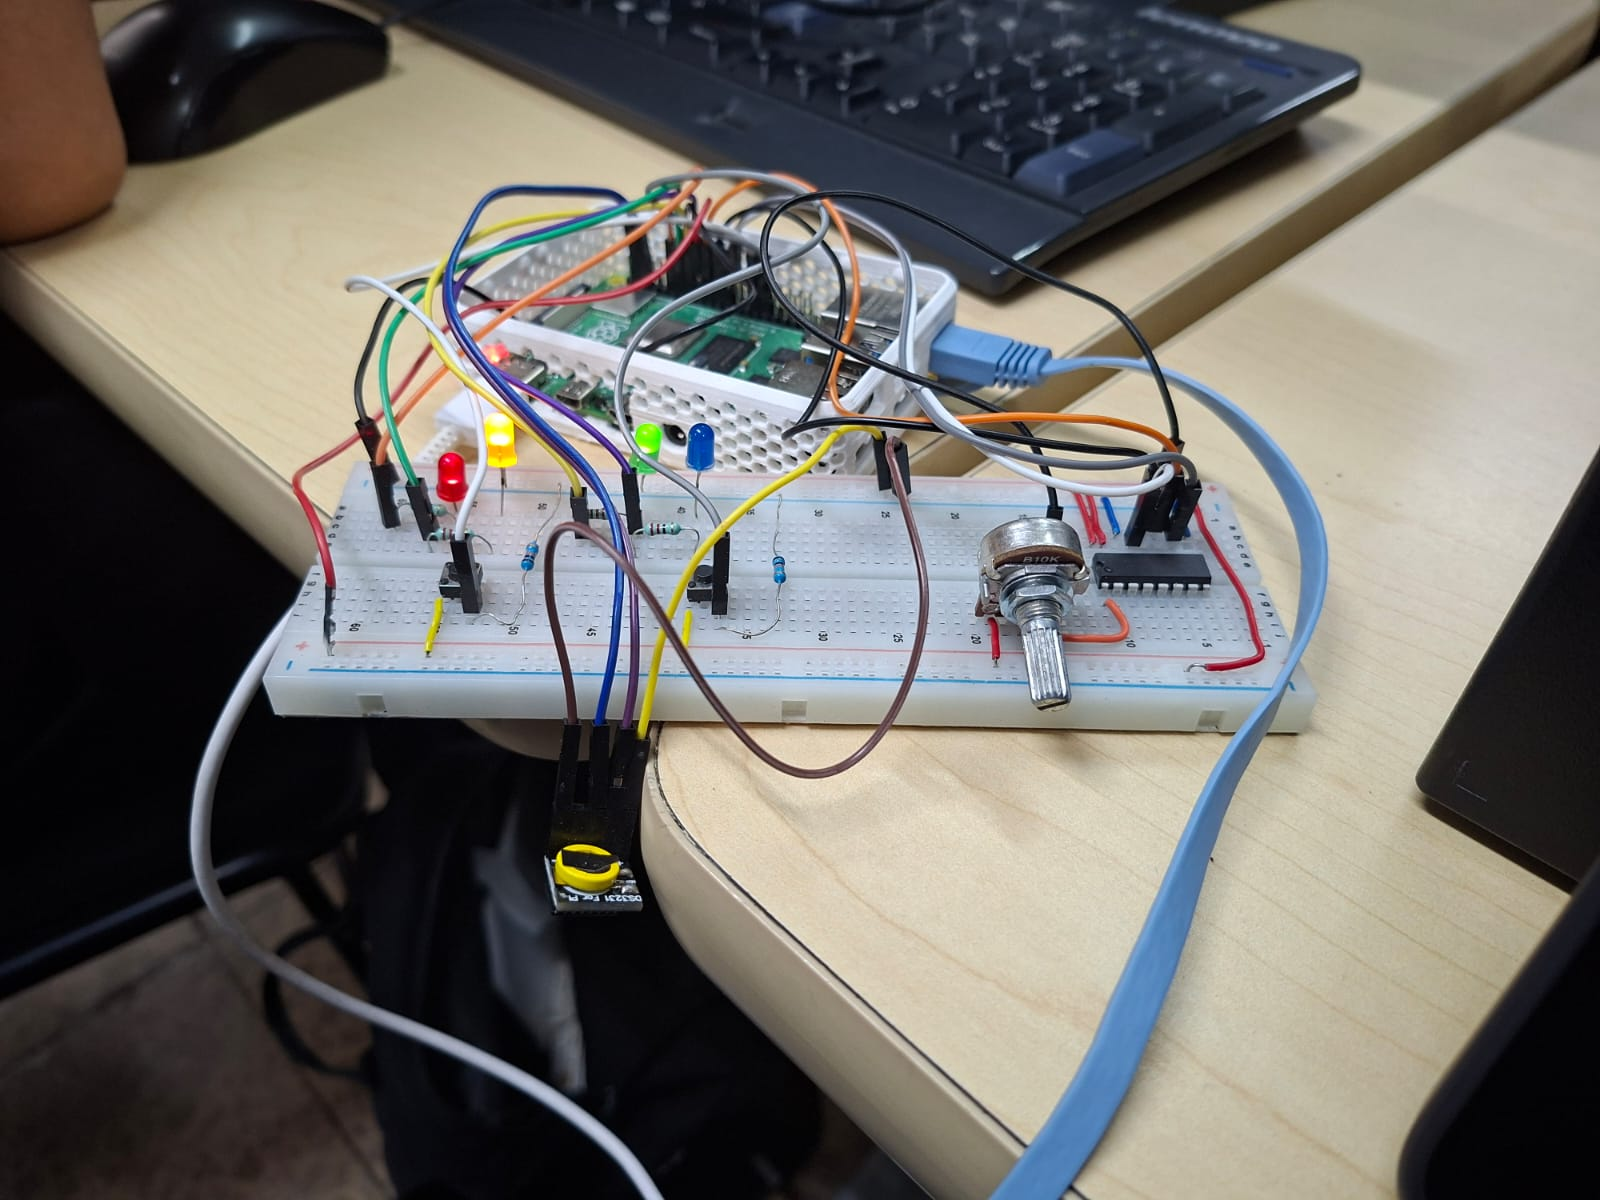
\includegraphics[width=0.8\columnwidth]{C_03_circuito_led_alarma.jpg}
	\caption{Circuito físico de la Raspberry Pi mostrando el estado de alarma con los LEDs encendidos.}
	\label{fig:c3}
\end{figure}

\begin{figure}[!ht]
	\centering
	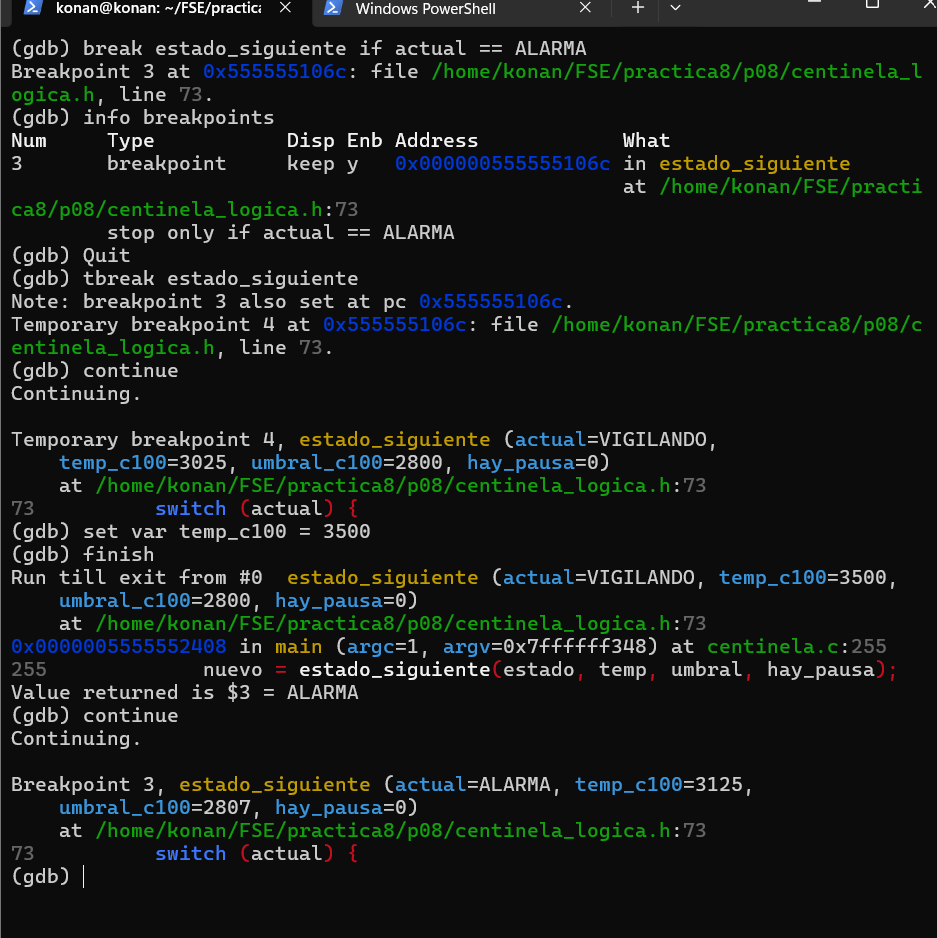
\includegraphics[width=0.9\columnwidth]{C_04_break_condicional_alarma.png}
	\caption{Creación de un breakpoint condicional (\texttt{actual == ALARMA}).}
	\label{fig:c4}
\end{figure}

\begin{figure}[!ht]
	\centering
	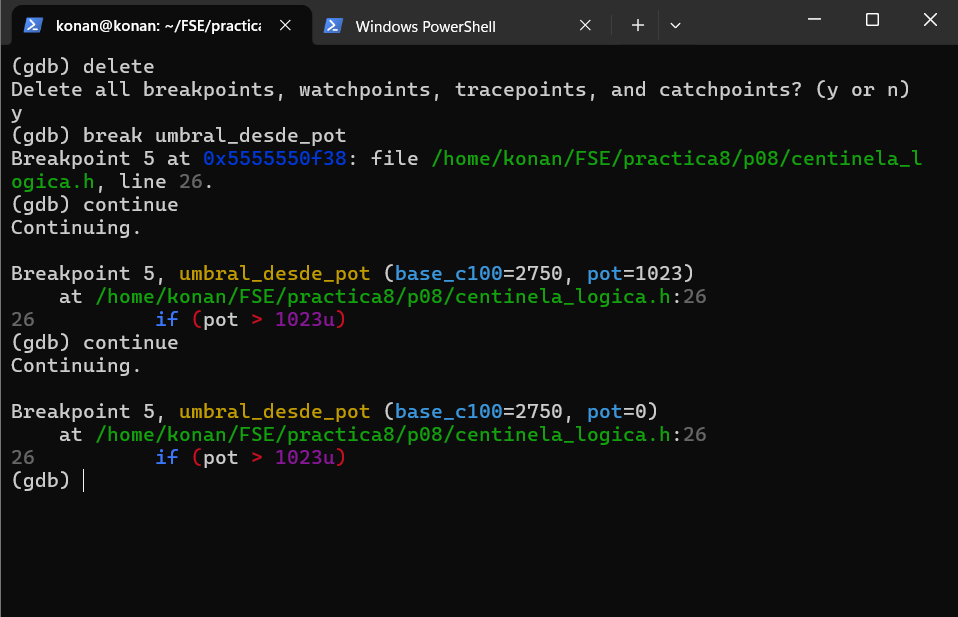
\includegraphics[width=0.9\columnwidth]{C_05_potenciometro_min_max.png}
	\caption{Breakpoint en \texttt{umbral\_desde\_pot} con el potenciómetro en mínimo y máximo.}
	\label{fig:c5}
\end{figure}

\begin{figure}[!ht]
	\centering
	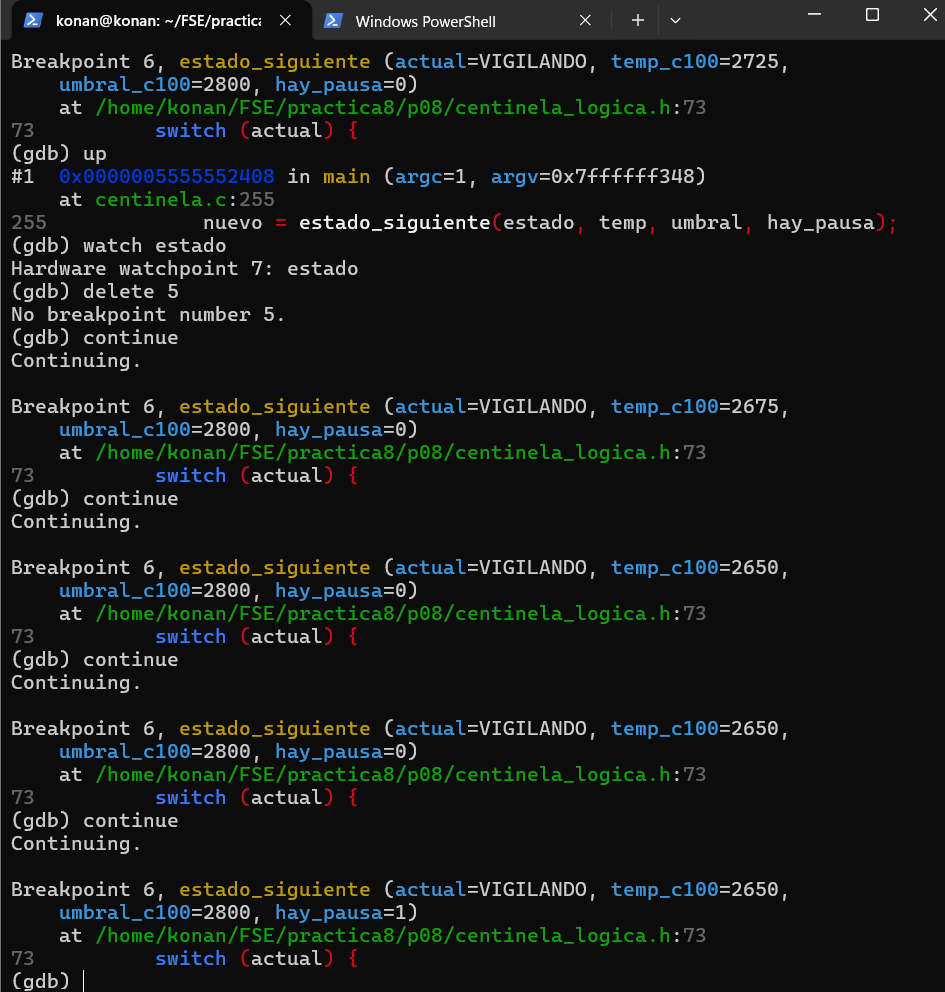
\includegraphics[width=0.9\columnwidth]{C_06_watch_estado_preparacion.png}
	\caption{Preparación del watchpoint en la variable de estado.}
	\label{fig:c6}
\end{figure}

\begin{figure}[!ht]
	\centering
	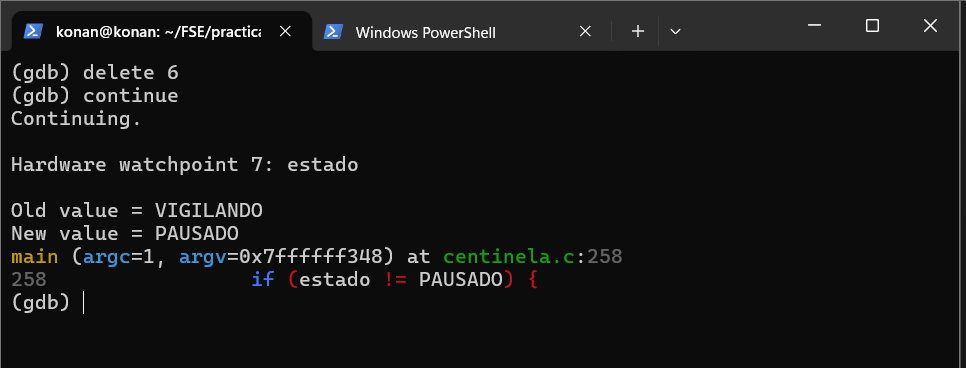
\includegraphics[width=0.9\columnwidth]{C_07_watch_estado_parada1.png}
	\caption{Primera detención del watchpoint mostrando el cambio de estado.}
	\label{fig:c7}
\end{figure}

\begin{figure}[!ht]
	\centering
	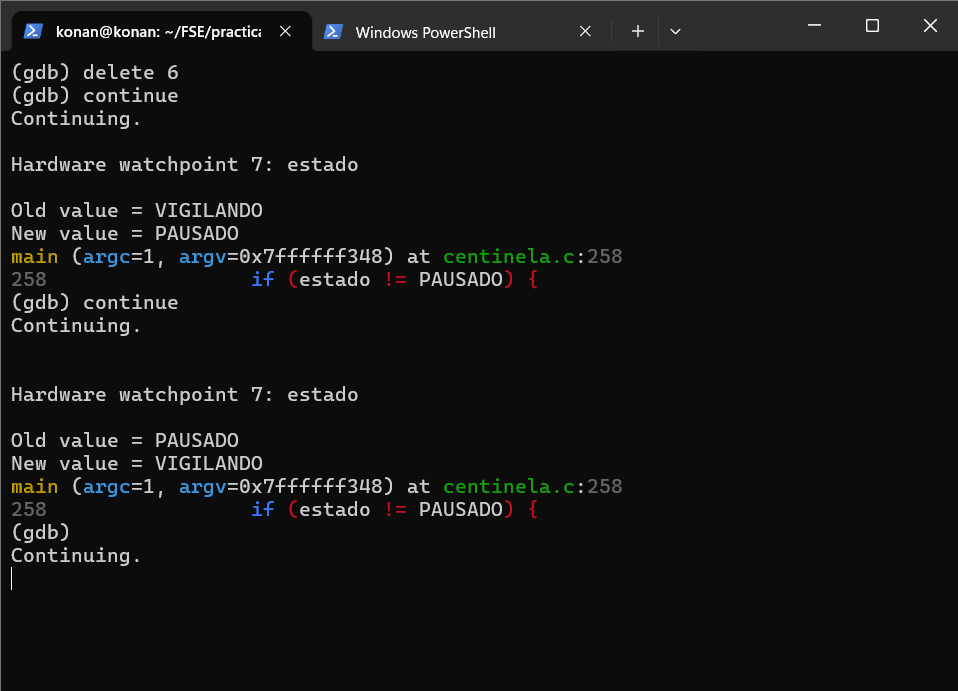
\includegraphics[width=0.9\columnwidth]{C_08_watch_estado_parada2.png}
	\caption{Segunda detención del watchpoint mostrando el cambio de estado.}
	\label{fig:c8}
\end{figure}

\subsection{Parte D. Tres fallas}
Se analizaron los tres programas proporcionados en el kit:
\begin{itemize}
	\item \textbf{f1\_nulo}: El programa sufre un \textit{Segmentation fault} (Figura~\ref{fig:d1}). Al usar \texttt{bt} y \texttt{info locals}, se observa que el puntero \texttt{pico} apunta a \texttt{0x0}. El error ocurre al hacer \texttt{printf} sin verificar si hubo lecturas válidas. \textbf{Corrección}: Validar que el contador de lecturas válidas sea mayor a cero antes de imprimir.
	\item \textbf{f2\_bucle}: El programa entra en un ciclo infinito (Figura~\ref{fig:d2}). Al interrumpirlo con Ctrl+C y usar \texttt{bt}, se observa que se queda atrapado en la función \texttt{ponderado}. \textbf{Corrección}: La variable iteradora se ve afectada por una condición de desbordamiento o un incremento erróneo dentro del ciclo que impide que se alcance la condición de término.
	\item \textbf{f3\_corrupcion}: La variable \texttt{cfg.umbral} cambia a un valor gigante. Usando un \textit{watchpoint} en \texttt{cfg.umbral}, \texttt{gdb} detiene la ejecución dentro de la función \texttt{strcpy} (Figura~\ref{fig:d3}). \textbf{Corrección}: La cadena \texttt{nombre} sobreescribe el límite del arreglo \texttt{etiqueta}, corrompiendo el campo contiguo \texttt{umbral}. Se debe usar \texttt{strncpy} o limitar el tamaño de la copia.
\end{itemize}

\begin{figure}[!ht]
	\centering
	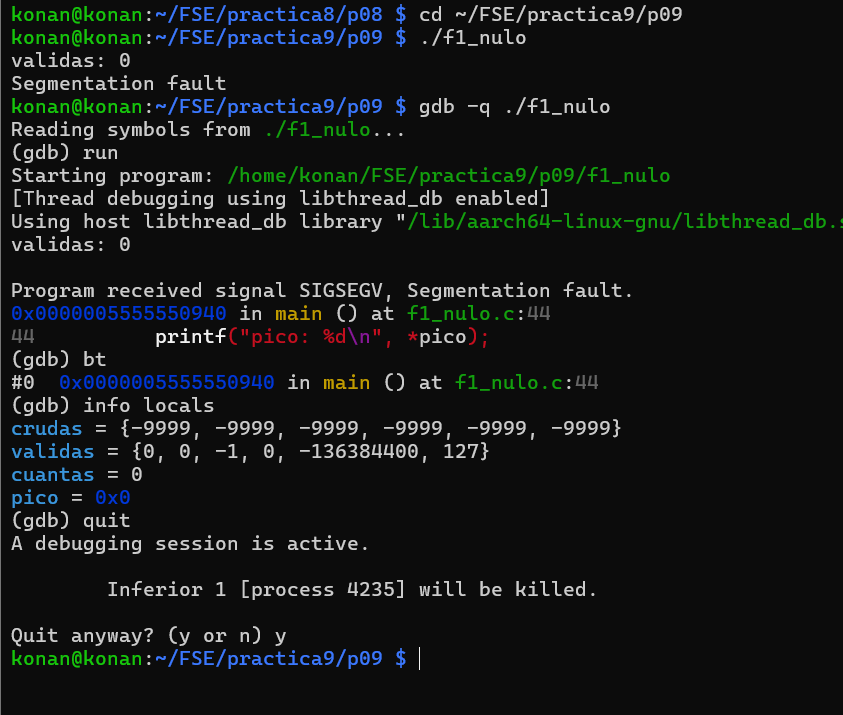
\includegraphics[width=0.9\columnwidth]{D_01_f1_nulo.png}
	\caption{Diagnóstico de \texttt{f1\_nulo}: Segmentation fault por puntero NULL.}
	\label{fig:d1}
\end{figure}

\begin{figure}[!ht]
	\centering
	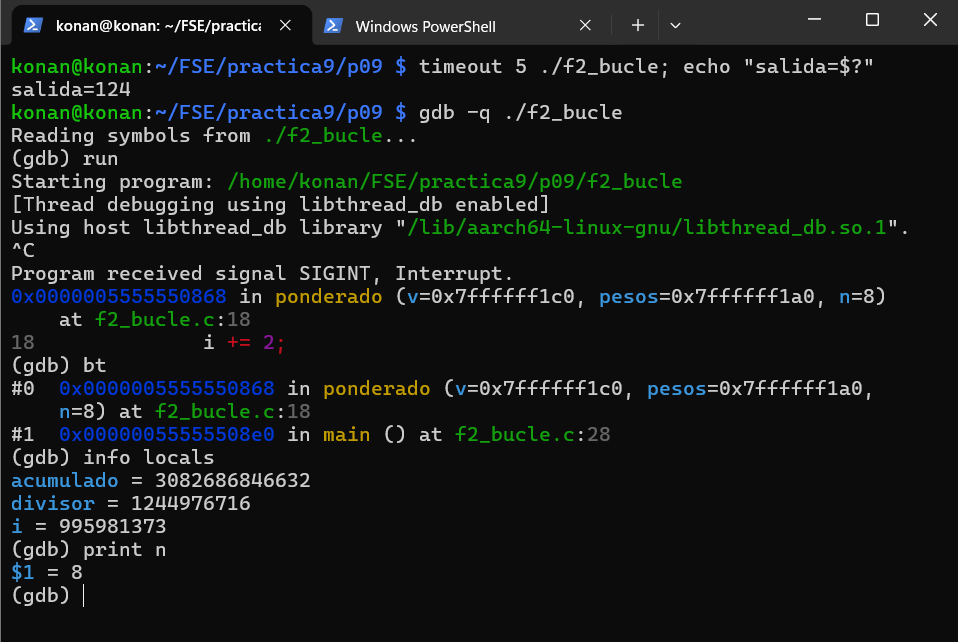
\includegraphics[width=0.9\columnwidth]{D_02_f2_bucle.png}
	\caption{Diagnóstico de \texttt{f2\_bucle}: interrupción manual y backtrace en el ciclo infinito.}
	\label{fig:d2}
\end{figure}

\begin{figure}[!ht]
	\centering
	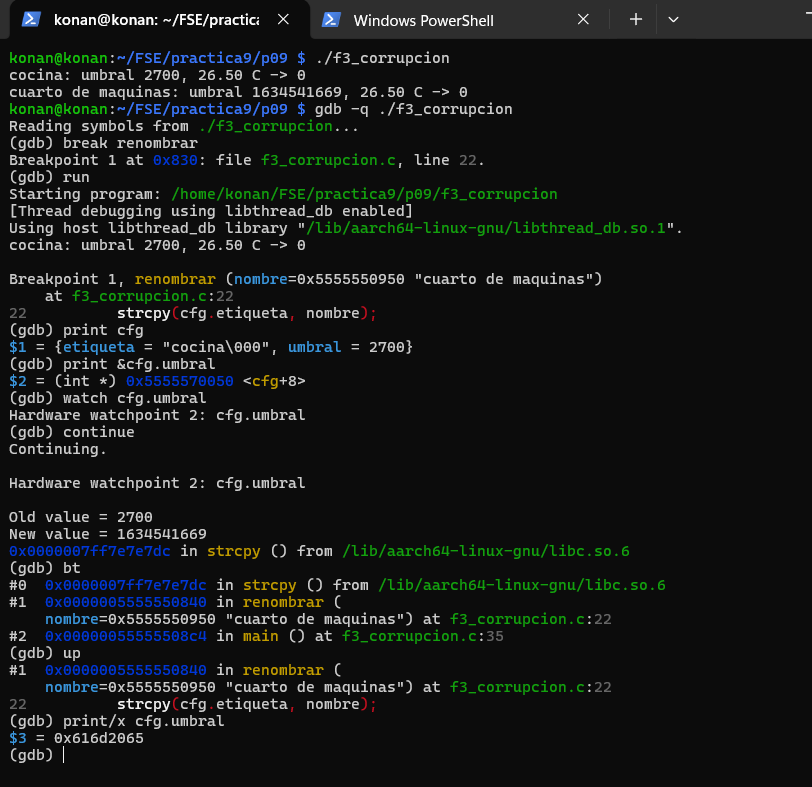
\includegraphics[width=0.9\columnwidth]{D_03_f3_corrupcion.png}
	\caption{Diagnóstico de \texttt{f3\_corrupcion}: el watchpoint revela el desbordamiento en \texttt{strcpy}.}
	\label{fig:d3}
\end{figure}

\subsection{Parte E. VS Code}
Se configuró el entorno gráfico instalando la extensión C/C++ de Microsoft en la Raspberry Pi. Se crearon los archivos \texttt{tasks.json} (para compilar con \texttt{make}) y \texttt{launch.json} (para lanzar \texttt{gdb}). Desde la interfaz, se colocaron \textit{breakpoints} y se avanzó con F10/F11 observando los paneles de Variables y Call Stack (Figuras~\ref{fig:e1} a \ref{fig:e4}).

\begin{figure}[!ht]
	\centering
	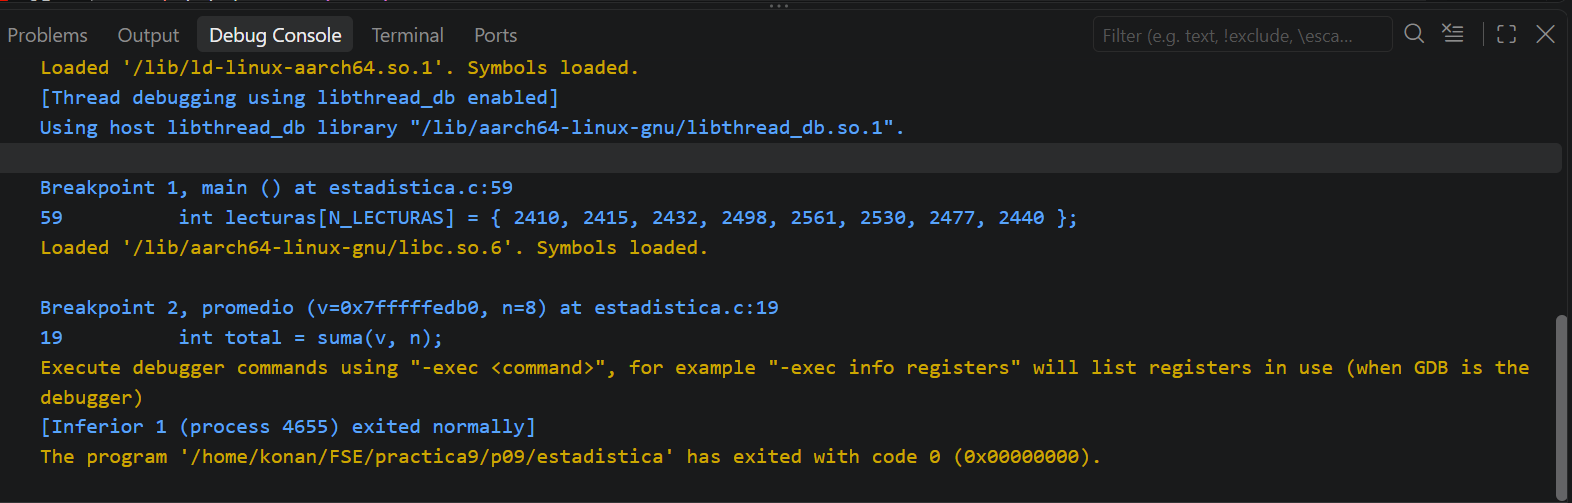
\includegraphics[width=0.9\columnwidth]{E_01_debug_console_f5.png}
	\caption{Consola de depuración de VS Code tras iniciar con F5.}
	\label{fig:e1}
\end{figure}

\begin{figure}[!ht]
	\centering
	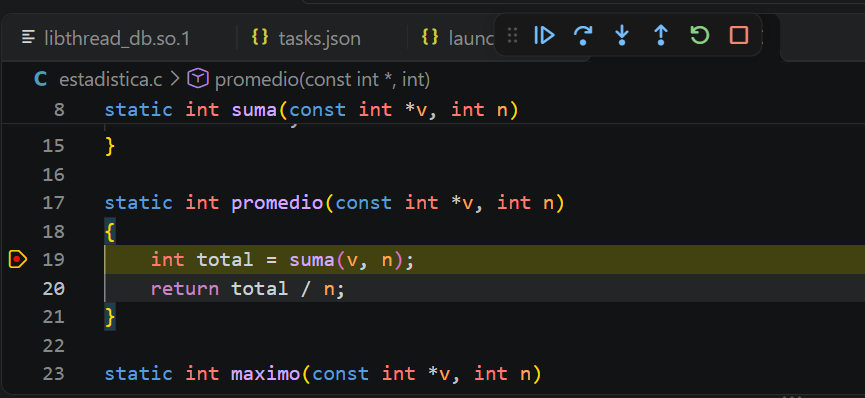
\includegraphics[width=0.9\columnwidth]{E_02_detenido_linea19.png}
	\caption{Programa detenido en la línea 19 desde la interfaz de VS Code.}
	\label{fig:e2}
\end{figure}

\begin{figure}[!ht]
	\centering
	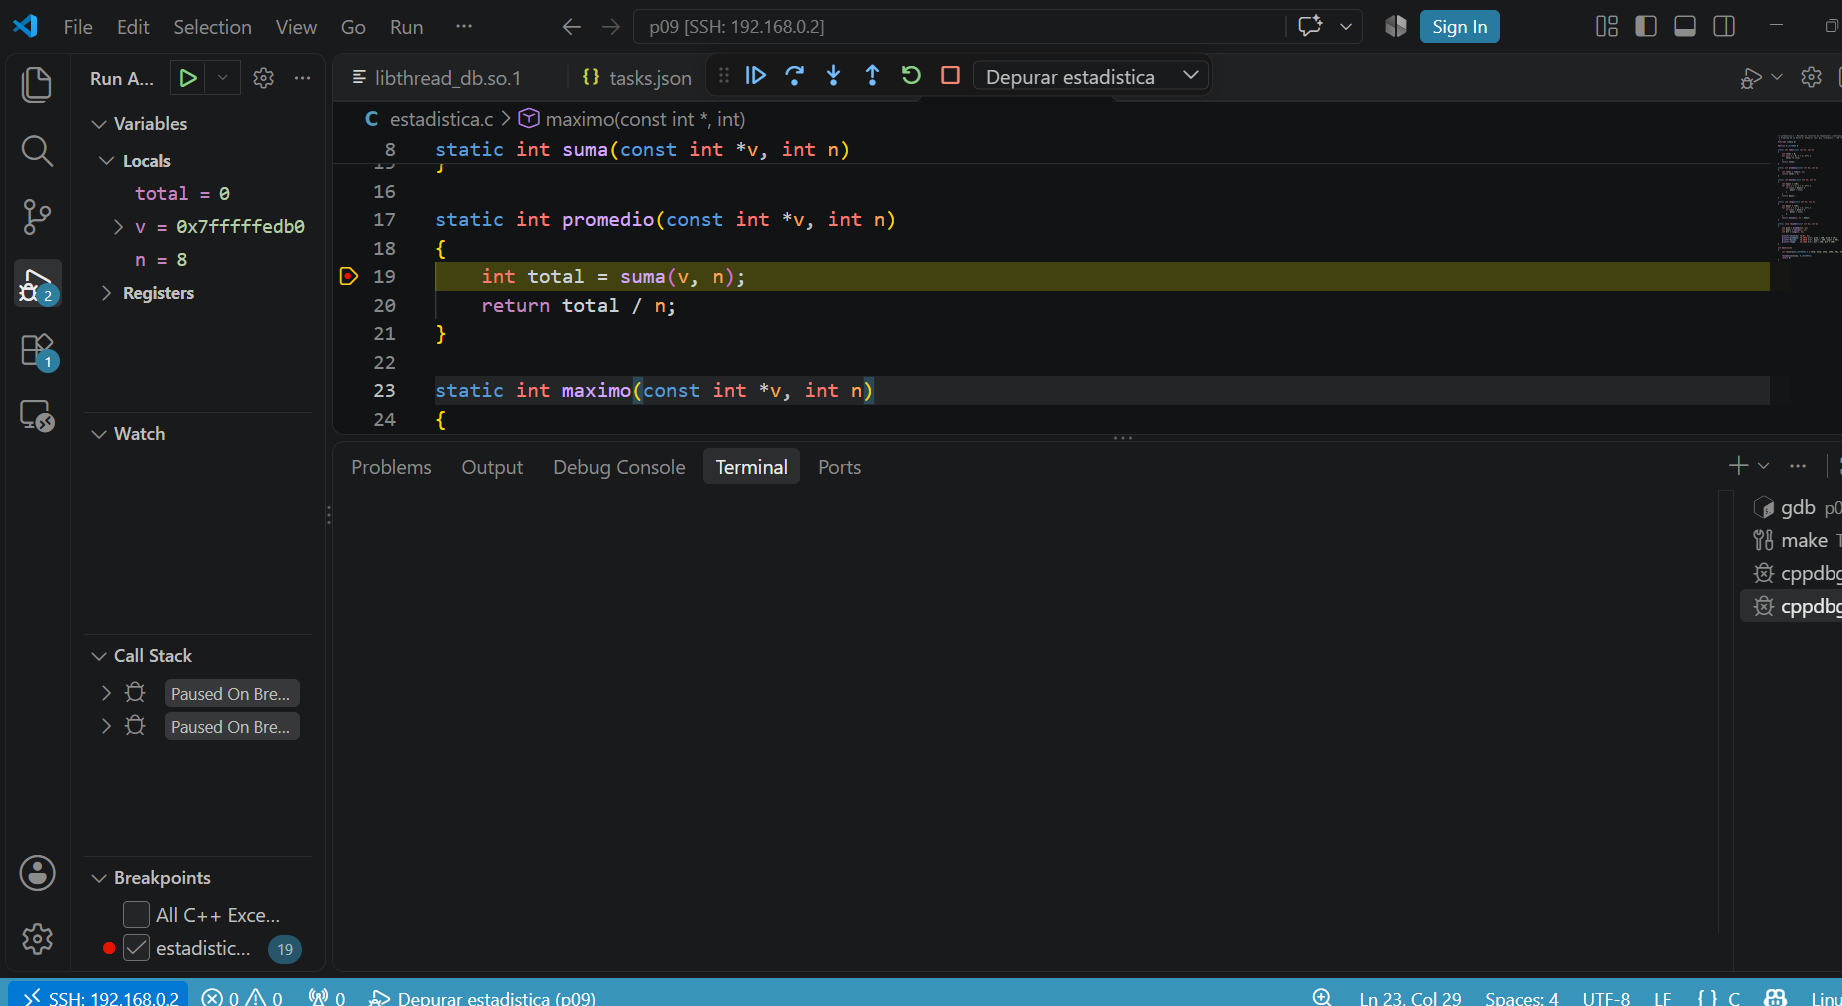
\includegraphics[width=0.9\columnwidth]{E_03_variables_callstack.png}
	\caption{Paneles de Variables y Call Stack en VS Code.}
	\label{fig:e3}
\end{figure}

\begin{figure}[!ht]
	\centering
	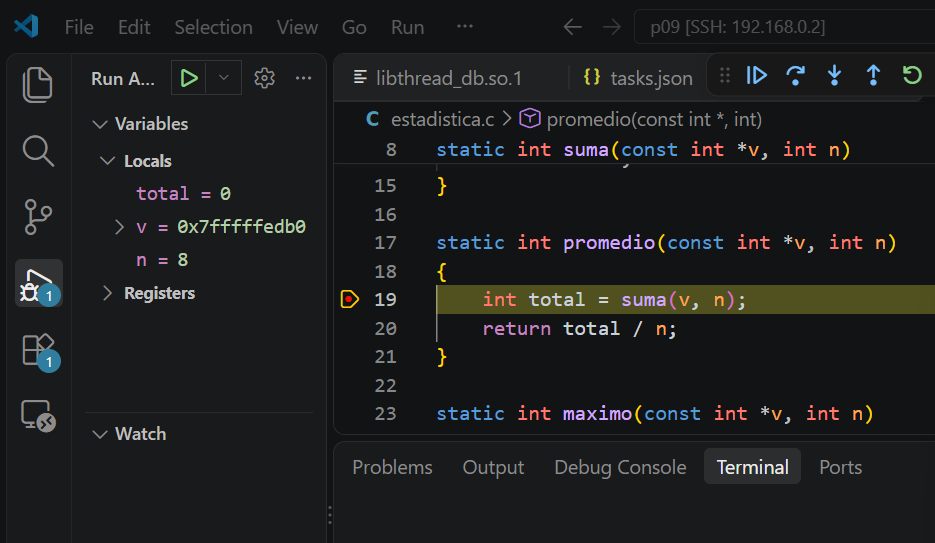
\includegraphics[width=0.9\columnwidth]{E_04_variables_locals.png}
	\caption{Inspección de variables locales en el depurador de VS Code.}
	\label{fig:e4}
\end{figure}

\subsection{Parte F. gdbserver}
Se abrieron dos sesiones SSH. En la primera se lanzó el programa con \texttt{gdbserver localhost:2345 ./centinela\_dbg}. En la segunda se abrió \texttt{gdb ./centinela\_dbg} y se conectó usando \texttt{target remote localhost:2345} (Figura~\ref{fig:f1}). Se comprobó que los comandos se ejecutan en la segunda terminal, mientras que la salida del programa y los mensajes de hardware aparecen en la primera.

\begin{figure}[!ht]
	\centering
	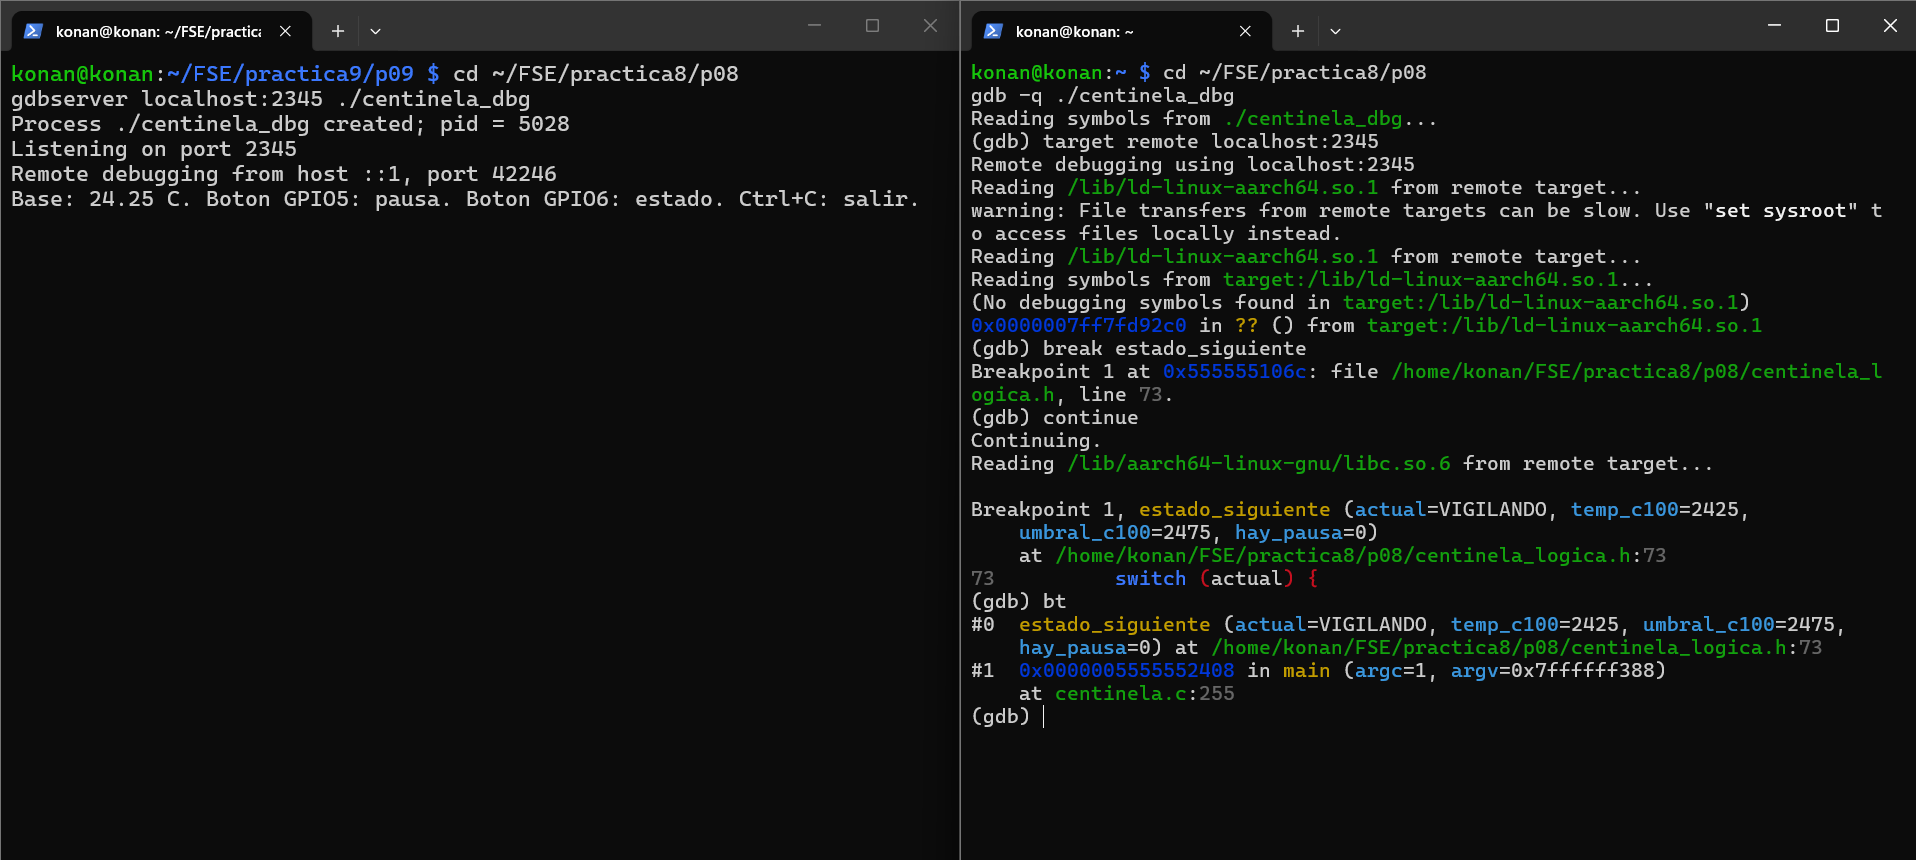
\includegraphics[width=0.9\columnwidth]{F_01_gdbserver_dos_terminales.png}
	\caption{Conexión remota con \texttt{gdbserver} y depuración desde otra terminal SSH.}
	\label{fig:f1}
\end{figure}

\subsection{Parte G. Reto: averiado}
Se analizó el programa \texttt{averiado.c}, el cual presentaba fallos en su lógica. Al ejecutarlo con \texttt{timeout 10 ./averiado}, se observó un \textit{Segmentation fault} tras unos segundos (Figura~\ref{fig:g1}). Depurando con \texttt{gdb}, se encontraron tres defectos (Figuras~\ref{fig:g2} a \ref{fig:g4}):
\begin{enumerate}
	\item \textbf{Defecto 1 (Falta de estado FALLA)}: El arreglo \texttt{nombre\_estado} solo tiene 3 elementos, pero el enum tiene 4. Al intentar acceder al índice 3 (FALLA), se lee memoria inválida (NULL), causando el \textit{Segmentation fault} (Figura~\ref{fig:g2}).
	\item \textbf{Defecto 2 (Índice del búfer circular)}: La línea \texttt{w->pos = (w->pos + 1) \% (VENTANA + 1);} debe ser módulo \texttt{VENTANA}. Al usar \texttt{VENTANA + 1}, el índice puede llegar a 4, corrompiendo la memoria fuera del arreglo de 4 elementos (Figura~\ref{fig:g3}).
	\item \textbf{Defecto 3 (Lógica de Histéresis)}: La condición para volver a VIGILANDO decía \texttt{temp >= UMBRAL - HISTERESIS}. Según las reglas, solo debe volver si es estrictamente menor o igual. Se corrigió a \texttt{temp > UMBRAL - HISTERESIS ? ALARMA : VIGILANDO;} (Figura~\ref{fig:g4}).
\end{enumerate}
La versión corregida (\texttt{averiado\_corregido.c}) se ejecutó exitosamente sin errores, comparando su salida con la original (Figura~\ref{fig:g5}) y mostrando el código final corregido (Figura~\ref{fig:g6}).

\begin{figure}[!ht]
	\centering
	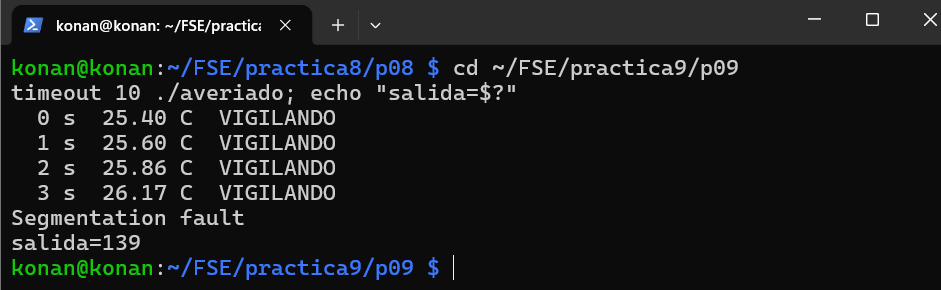
\includegraphics[width=0.9\columnwidth]{G_01_averiado_original_segfault.png}
	\caption{Ejecución de \texttt{averiado.c} mostrando el Segmentation fault.}
	\label{fig:g1}
\end{figure}

\begin{figure}[!ht]
	\centering
	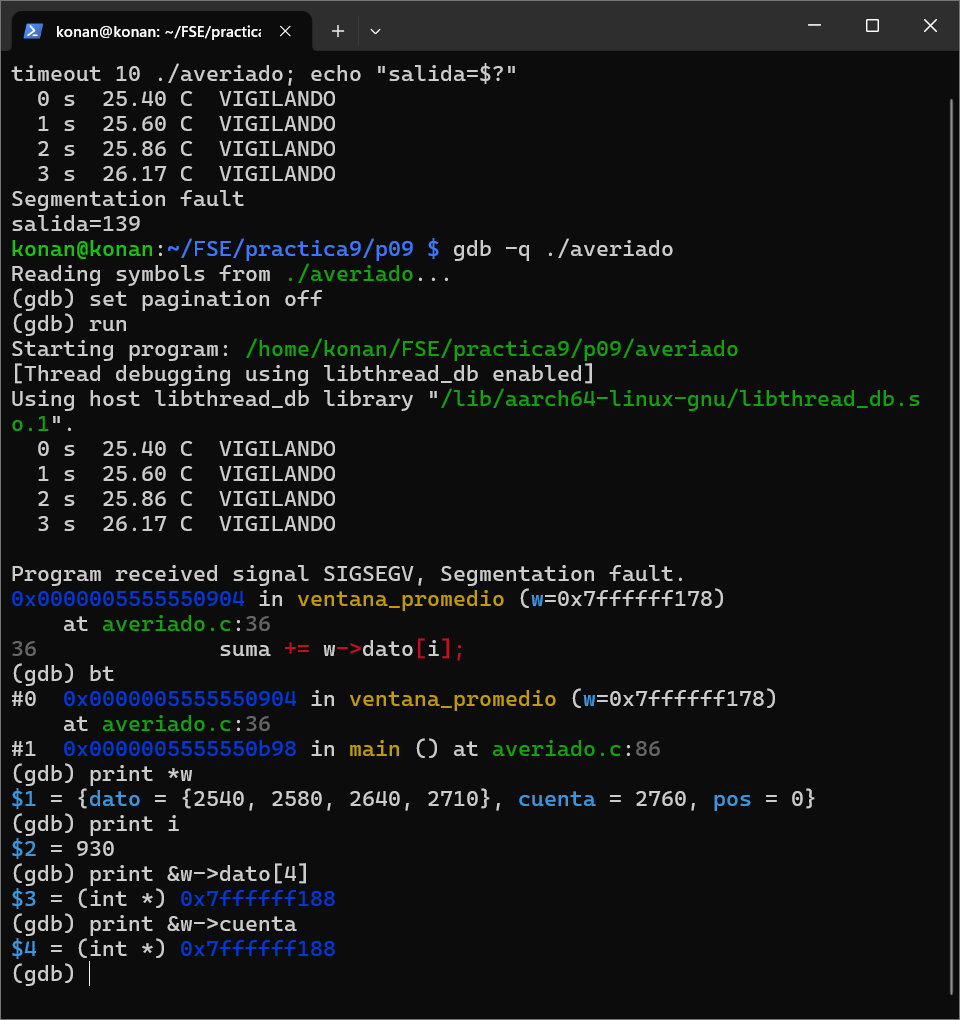
\includegraphics[width=0.9\columnwidth]{G_02_defecto1_ventana.png}
	\caption{Backtrace (\texttt{bt}) mostrando el fallo en \texttt{strcpy} por puntero nulo (Defecto 1).}
	\label{fig:g2}
\end{figure}

\begin{figure}[!ht]
	\centering
	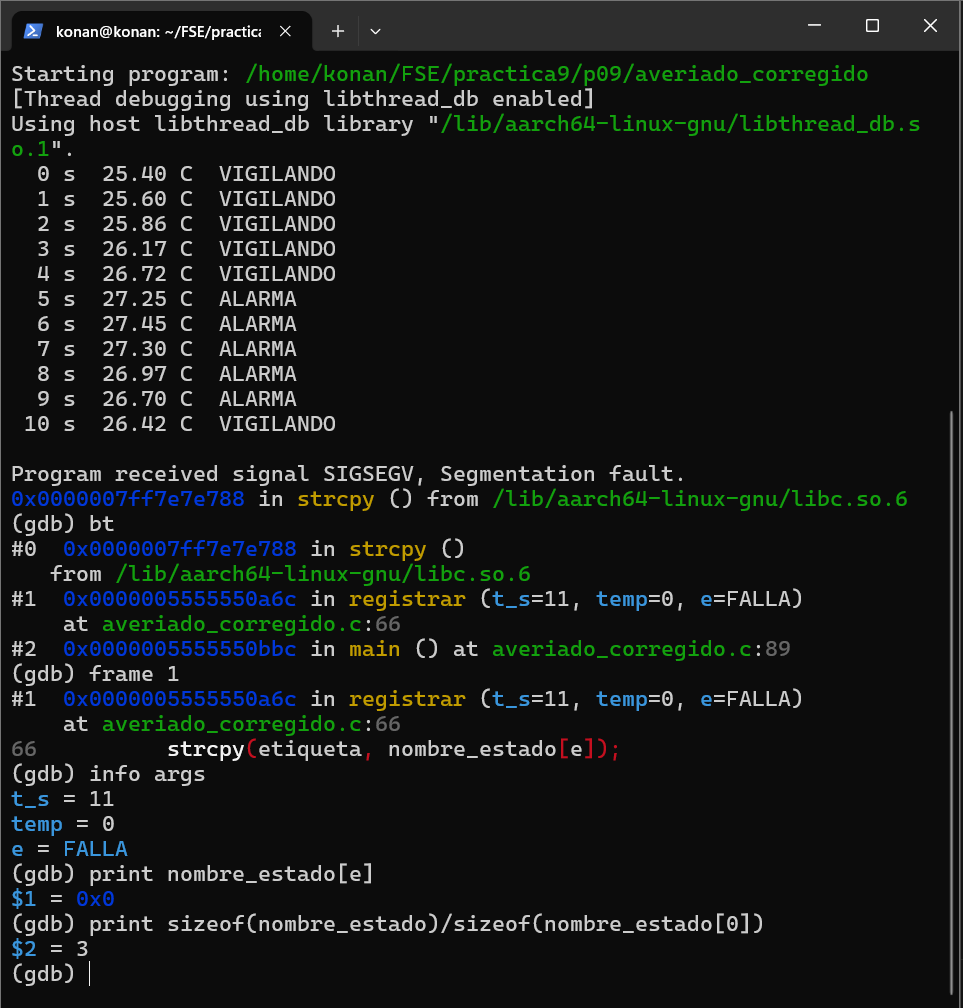
\includegraphics[width=0.9\columnwidth]{G_03_defecto2_nombre_falla.png}
	\caption{Análisis del índice del búfer circular (Defecto 2).}
	\label{fig:g3}
\end{figure}

\begin{figure}[!ht]
	\centering
	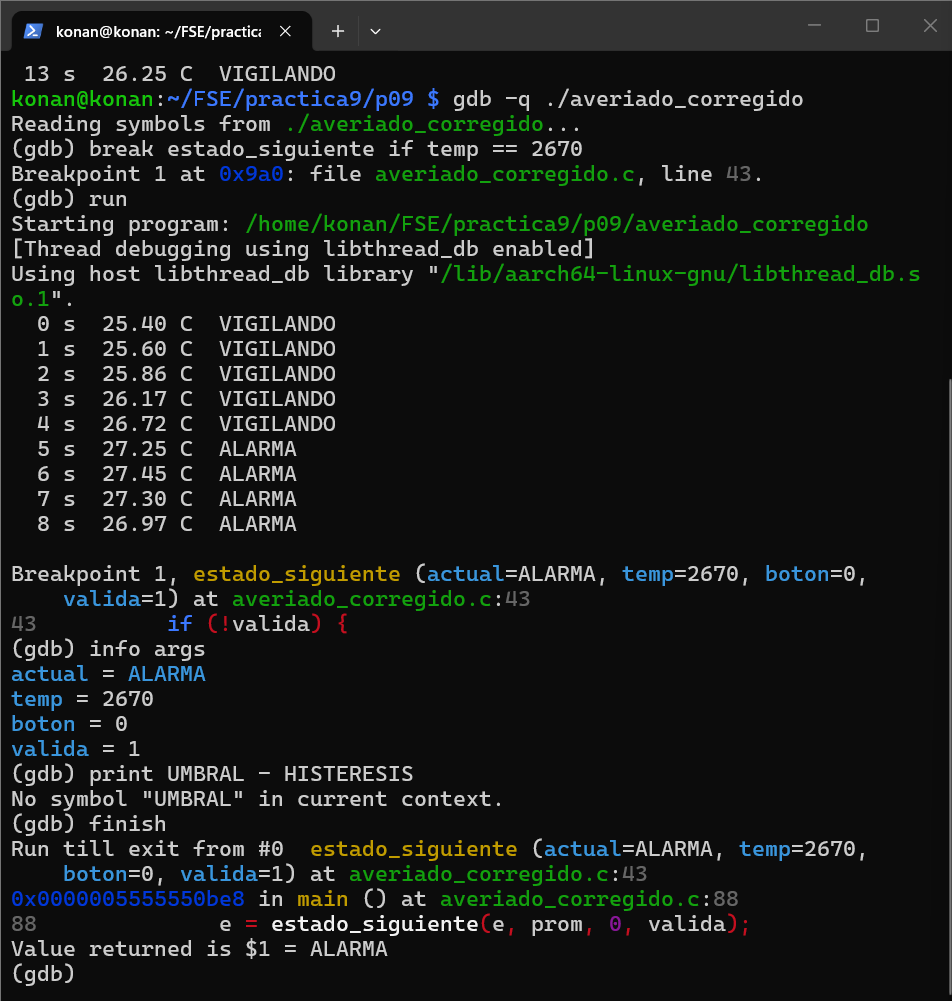
\includegraphics[width=0.9\columnwidth]{G_04_defecto3_histeresis.png}
	\caption{Depuración de la lógica de histéresis (Defecto 3).}
	\label{fig:g4}
\end{figure}

\begin{figure}[!ht]
	\centering
	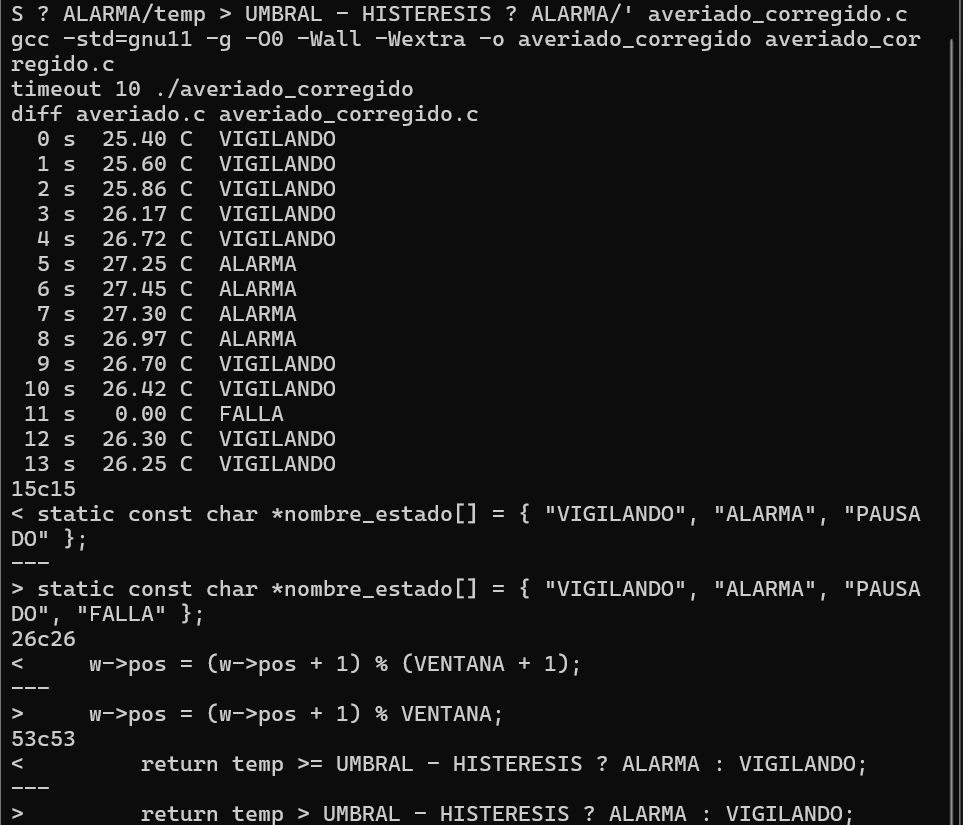
\includegraphics[width=0.9\columnwidth]{G_05_corregido_salida_diff.png}
	\caption{Comparación (\texttt{diff}) de los cambios y ejecución exitosa de \texttt{averiado\_corregido.c}.}
	\label{fig:g5}
\end{figure}

\begin{figure}[!ht]
	\centering
	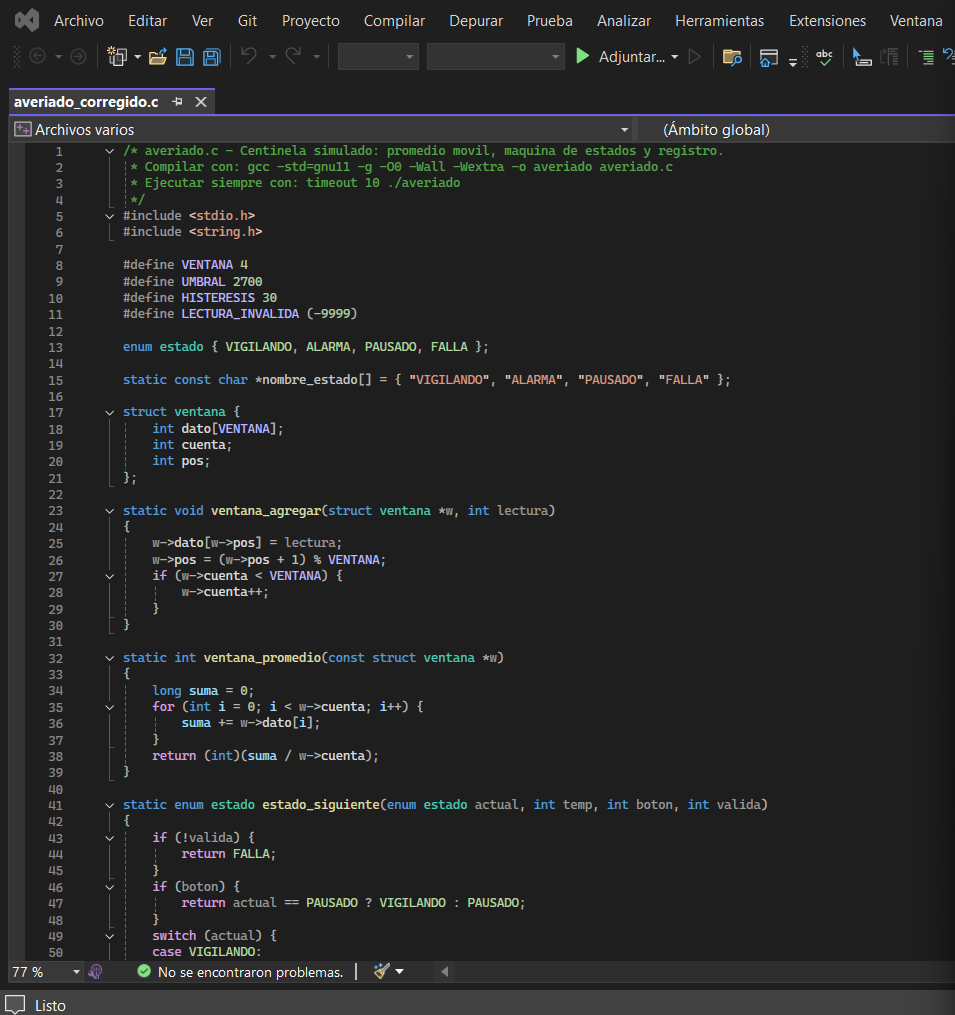
\includegraphics[width=0.9\columnwidth]{G_06_averiado_corregido_codigo.png}
	\caption{Código de \texttt{averiado\_corregido.c} en VS Code mostrando las correcciones.}
	\label{fig:g6}
\end{figure}

% ---------------------------------------------------------
% SECCIÓN IV: RESULTADOS Y ANÁLISIS
% ---------------------------------------------------------
\section{Resultados y Análisis}

\subsection{Preguntas Parte B (gdb en terminal)}
\textbf{¿Qué diferencia hay entre \texttt{next} y \texttt{step} en esa línea y qué habrías visto si usaras \texttt{finish} en lugar de \texttt{step}?} \\
\texttt{next} ejecuta la instrucción actual sin entrar en las funciones llamadas. \texttt{step} sí entra en la función, mostrando el código interno de \texttt{suma}. Si se hubiera usado \texttt{finish} en lugar de \texttt{step}, el depurador habría terminado la ejecución de \texttt{suma} inmediatamente y se habría detenido de nuevo en \texttt{promedio}, mostrando el valor total calculado (\(19763\)).

\subsection{Preguntas Parte C (Centinela)}
\textbf{Después de mantener el programa detenido 30 segundos, ¿qué muestra la columna de tiempo de centinela.csv en las líneas siguientes y por qué?} \\
Mostraría un salto de tiempo de 30 segundos o más respecto a la lectura anterior. Esto se debe a que, aunque el depurador detiene la ejecución del proceso en el espacio de usuario, el reloj del sistema (\textit{hardware}) sigue avanzando. Al reanudar el programa, la siguiente llamada a \texttt{time(NULL)} obtendrá el tiempo real actual, reflejando el tiempo que el programa estuvo pausado.

\subsection{Preguntas Parte E (VS Code)}
\textbf{¿En qué situaciones de un sistema embebido conviene un \textit{logpoint} en lugar de un \textit{breakpoint}?} \\
Un \textit{logpoint} es ideal cuando se necesita monitorear el comportamiento del sistema (como el valor de un sensor o el estado de una máquina) durante periodos prolongados o en tiempo real sin interrumpir el flujo del programa. Detener el programa con un \textit{breakpoint} puede causar que se pierdan eventos, se desborden búferes de hardware o se interrumpa una comunicación crítica.

\subsection{Preguntas Parte F (gdbserver)}
\textbf{¿Qué pasos adicionales exige compilar en la laptop y depurar en la Pi, y por qué se usa \texttt{gdbserver} en sistemas con pocos recursos?} \\
Requiere compilar con una herramienta de compilación cruzada (\textit{cross-compiler}) en la laptop, transferir el binario a la Pi y asegurarse de que las bibliotecas compartidas coincidan. Se usa \texttt{gdbserver} porque consume mucha menos memoria y CPU en el sistema objetivo en comparación con ejecutar el \texttt{gdb} completo. Además, permite aprovechar la interfaz gráfica o el mayor poder de procesamiento de una computadora host.

% ---------------------------------------------------------
% SECCIÓN V: CÓDIGO Y REPOSITORIO
% ---------------------------------------------------------
\section{Código Fuente y Repositorio}
Como evidencia del desarrollo y para cumplir con los entregables solicitados, todo el código fuente de esta práctica, incluyendo los archivos de configuración de VS Code (\texttt{launch.json} y \texttt{tasks.json}) y la versión corregida del reto, se encuentra alojado en el repositorio oficial del equipo:

\begin{center}
	\url{https://github.com/YizusDP/Practicas_Embebidos}
\end{center}

A continuación, se presenta un fragmento de la corrección aplicada a la función \texttt{estado\_siguiente} del archivo \texttt{averiado\_corregido.c}:

\begin{lstlisting}[language=C]
// Correccion en la logica de histeresis (Defecto 3)
if (actual == ALARMA) {
    // Se corrigio el operador logico para que solo baje a VIGILANDO
    // si la temperatura es ESTRICTAMENTE menor al umbral - histeresis
    if (temp > UMBRAL - HISTERESIS) {
        return ALARMA;
    } else {
        return VIGILANDO;
    }
}
\end{lstlisting}

% ---------------------------------------------------------
% SECCIÓN VI: CONCLUSIONES
% ---------------------------------------------------------
\section{Conclusiones}

\textbf{Belmont Muñoz Samuel.} \\
Esta práctica demostró la importancia del uso del depurador en el desarrollo embebido. Aprender a usar \texttt{breakpoints} condicionales y \textit{watchpoints} permitió identificar fallos lógicos y de memoria sin necesidad de saturar el código con \texttt{printfs}. La integración de VS Code a través de SSH proporciona un entorno de desarrollo muy cómodo, aunque el dominio de \texttt{gdb} por terminal sigue siendo vital para el análisis a bajo nivel.

\textbf{Domínguez Palacios Jesús Alejandro.} \\
Comprendí que el comportamiento del hardware y el software están desacoplados durante la depuración. Al pausar el Centinela, los LEDs se quedan en su último estado, ignorando los cambios ambientales. El uso de \texttt{gdbserver} me pareció una herramienta fundamental para entornos reales donde el dispositivo puede no tener monitor ni teclado. Encontrar la corrupción de memoria en \texttt{f3\_corrupcion} con un \textit{watchpoint} fue el momento clave de la práctica, demostrando por qué la validación de tamaños es crucial.

\textbf{Dorantes Mejía Emmanuel.} \\
Esta práctica me ayudó a entender que la depuración no es solo buscar errores de sintaxis, sino analizar el estado del programa en tiempo real. Herramientas como los \textit{watchpoints} en \texttt{gdb} fueron clave para encontrar la corrupción de memoria en \texttt{f3\_corrupcion}, un error que a simple vista parecía que la variable cambiaba sola. Además, compilar con la bandera \texttt{-O0} me demostró que el compilador puede ocultar información valiosa si intentamos depurar código optimizado.

\textbf{García Olvera Emiliano.} \\
El uso de VS Code con Remote-SSH facilitó enormemente el proceso de depuración en la Raspberry Pi, haciendo que el análisis gráfico de variables y la pila de llamadas fuera mucho más intuitivo que en la terminal pura. Aprendí a configurar las tareas de compilación en \texttt{tasks.json} y la ejecución en \texttt{launch.json}. Por otro lado, el reto de \texttt{averiado.c} demostró que los errores lógicos, como el cálculo incorrecto de la histéresis o los índices del búfer circular, son tan críticos como los errores de memoria y requieren un análisis cuidadoso de las condiciones del código.

\textbf{Hernández Alonso Antonio Adonahí.} \\
El depurador es una herramienta que ahorra horas de trabajo. En esta práctica logré diagnosticar el bucle infinito de \texttt{f2\_bucle} interrumpiendo el proceso y revisando la pila de llamadas. También quedó claro que las optimizaciones del compilador (\texttt{-O0} frente a \texttt{-O2}) afectan directamente la depuración; sin la bandera \texttt{-O0}, el compilador reordena o elimina variables, dificultando el rastreo paso a paso. El reto \texttt{averiado} consolidó la teoría de estados e índices en C.

\textbf{Jiménez Reyes Alan Yael.} \\
A través de esta práctica logré identificar fallos complejos que a simple vista parecían errores lógicos simples. El error de segmentación de \texttt{f1\_nulo} y la corrupción por \texttt{strcpy} en \texttt{f3\_corrupcion} demuestran la fragilidad de C cuando no se validan los punteros y los límites de los arreglos. Aprender a configurar VS Code con \texttt{tasks.json} y \texttt{launch.json} me facilitará enormemente el desarrollo en proyectos futuros, automatizando la compilación y la depuración en la Raspberry Pi.

% ---------------------------------------------------------
% DECLARACIÓN DE IA Y REFERENCIAS
% ---------------------------------------------------------
\section*{Declaración de Uso de Inteligencia Artificial}
Se utilizó Claude (Anthropic) como herramienta de apoyo para la estructuración del reporte en LaTeX y la revisión de la redacción técnica. El equipo revisó, ejecutó, validó y analizó de forma independiente cada una de las herramientas de depuración (gdb, gdbserver y VS Code), así como los resultados obtenidos en la Raspberry Pi presentados en este documento.

\begin{thebibliography}{00}
	\bibitem{gdb_docs} Free Software Foundation. (2024). ``Debugging with GDB''. Disponible en: https://sourceware.org/gdb/documentation
	\bibitem{vscode_remote} Microsoft. (2024). ``Remote Development using SSH''. Disponible en: https://code.visualstudio.com/docs/remote/ssh
	\bibitem{vscode_cpp} Microsoft. (2024). ``Debugging C++ in Visual Studio Code''. Disponible en: https://code.visualstudio.com/docs/cpp/cpp-debug
	\bibitem{barr} Barr, M. y Massa, A. (2006). \textit{Programming Embedded Systems}, 2.ª ed. O'Reilly.
	\bibitem{kernighan} Kernighan, B. W. y Ritchie, D. M. (1988). \textit{The C Programming Language}, 2.ª ed. Prentice Hall.
    \bibitem Anthropic. (2026). “Claude”. Disponible en: https://claude.ai
\end{thebibliography}

\end{document}
